\documentclass[../../../main.tex]{subfiles}

\begin{document}
% do 4-5 alternatives

% 1. InvenTree
\paragraph{InvenTree}
\url{https://inventree.org/}\\


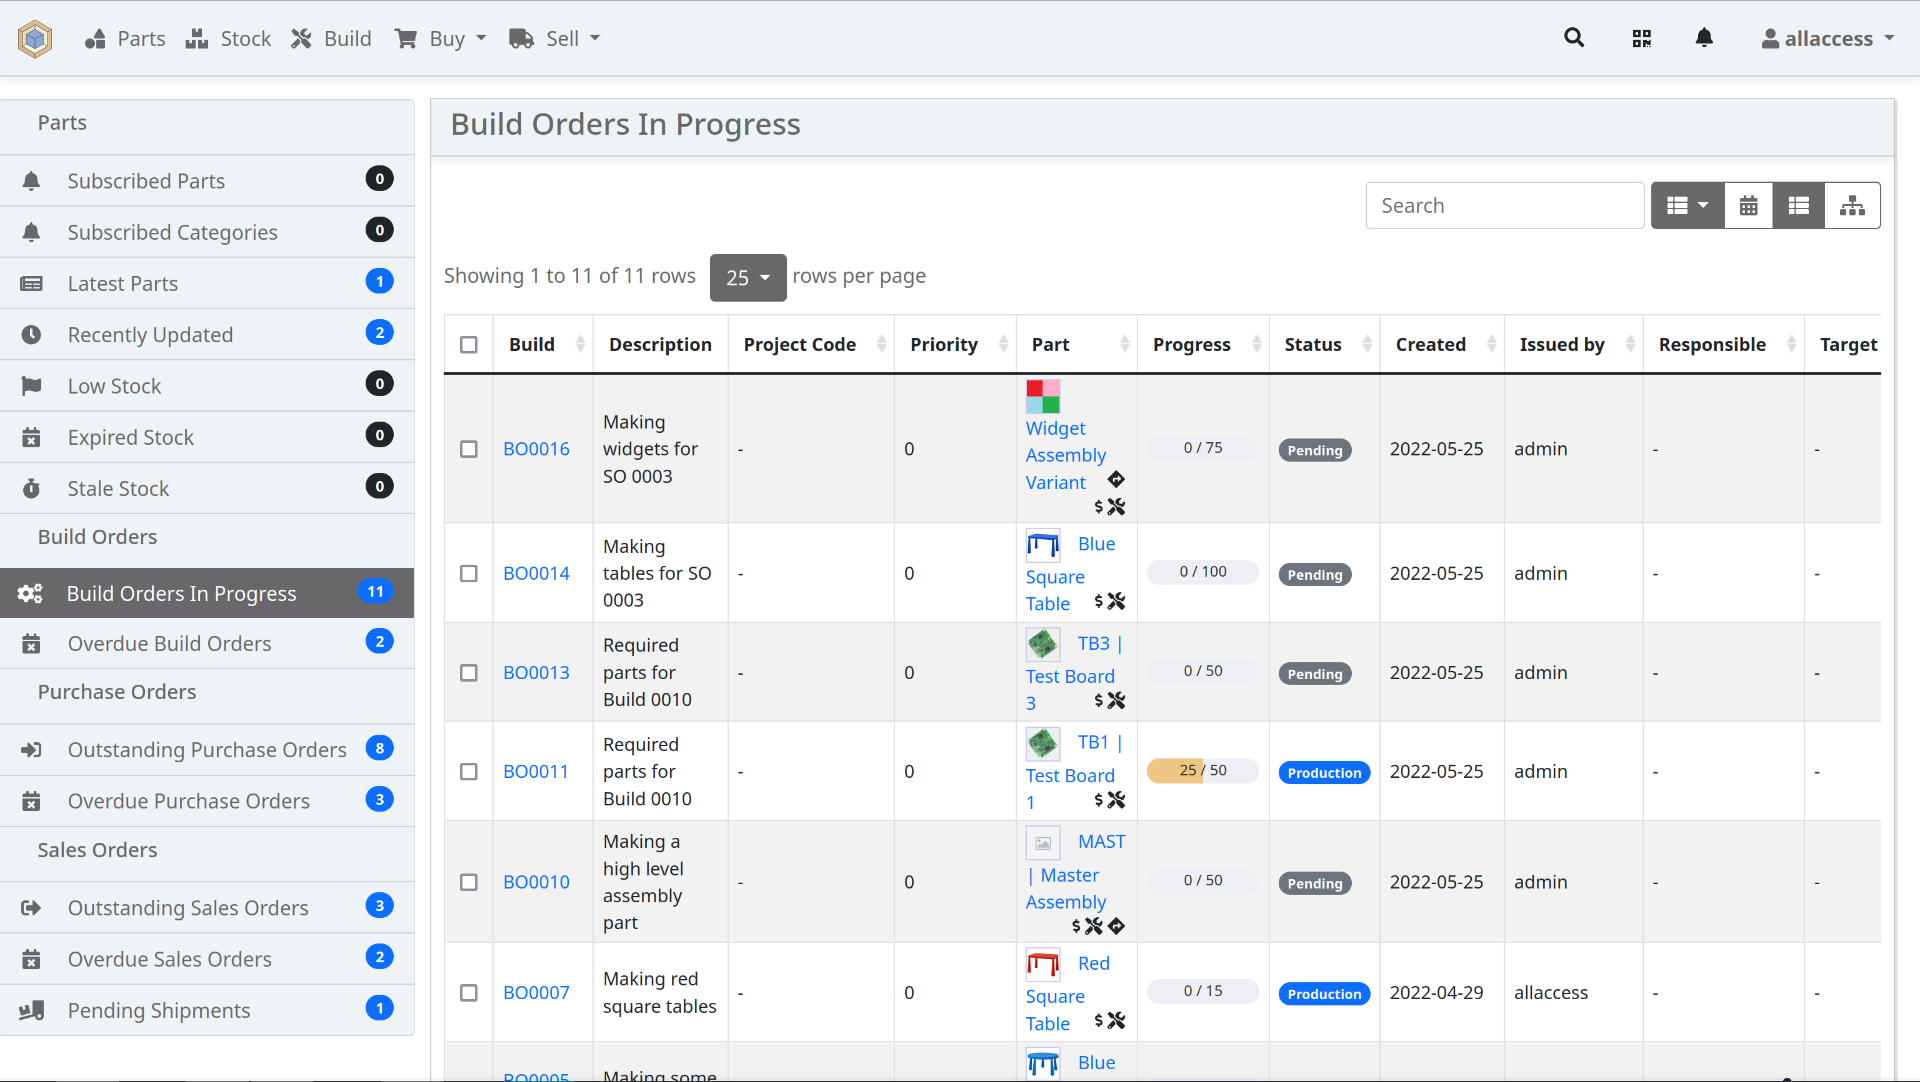
\includegraphics[width=15cm]{inventree_demo_homepage.png}

\subparagraph{Overview}

\noindent\\ InvenTree is an \textbf{open-source} inventory management system, providing \textit{low level stock control and part tracking}.
It uses a Python/Django database backend and provides both a \textbf{web-based interface} as well as a REST API for interacting with other services.
InvenTree also has a powerful plugin system for custom applications and other extensions. \\

\subparagraph{Parts applicable to my solution\\}

\begin{outline}
    \1 Web-based application\\
    \textit{The application will be web-based.}

    \1 Modern, Relatively simple user interface\\
    \textit{InvenTree offers a relatively simple and intuitive user interface.}
\end{outline}

\subparagraph{Parts \underline{not} applicable to my solution\\}

\begin{outline}
    \1 Stock control and part tracking specific features\\
    \textit{I am looking to implement a system that is capable of being far more generalized than just part tracking, although the system will have features for library book tracking.}
\end{outline}

\pagebreak

% 2. PartKeepr
\paragraph{PartKeepr}
\url{https://partkeepr.org/}\\

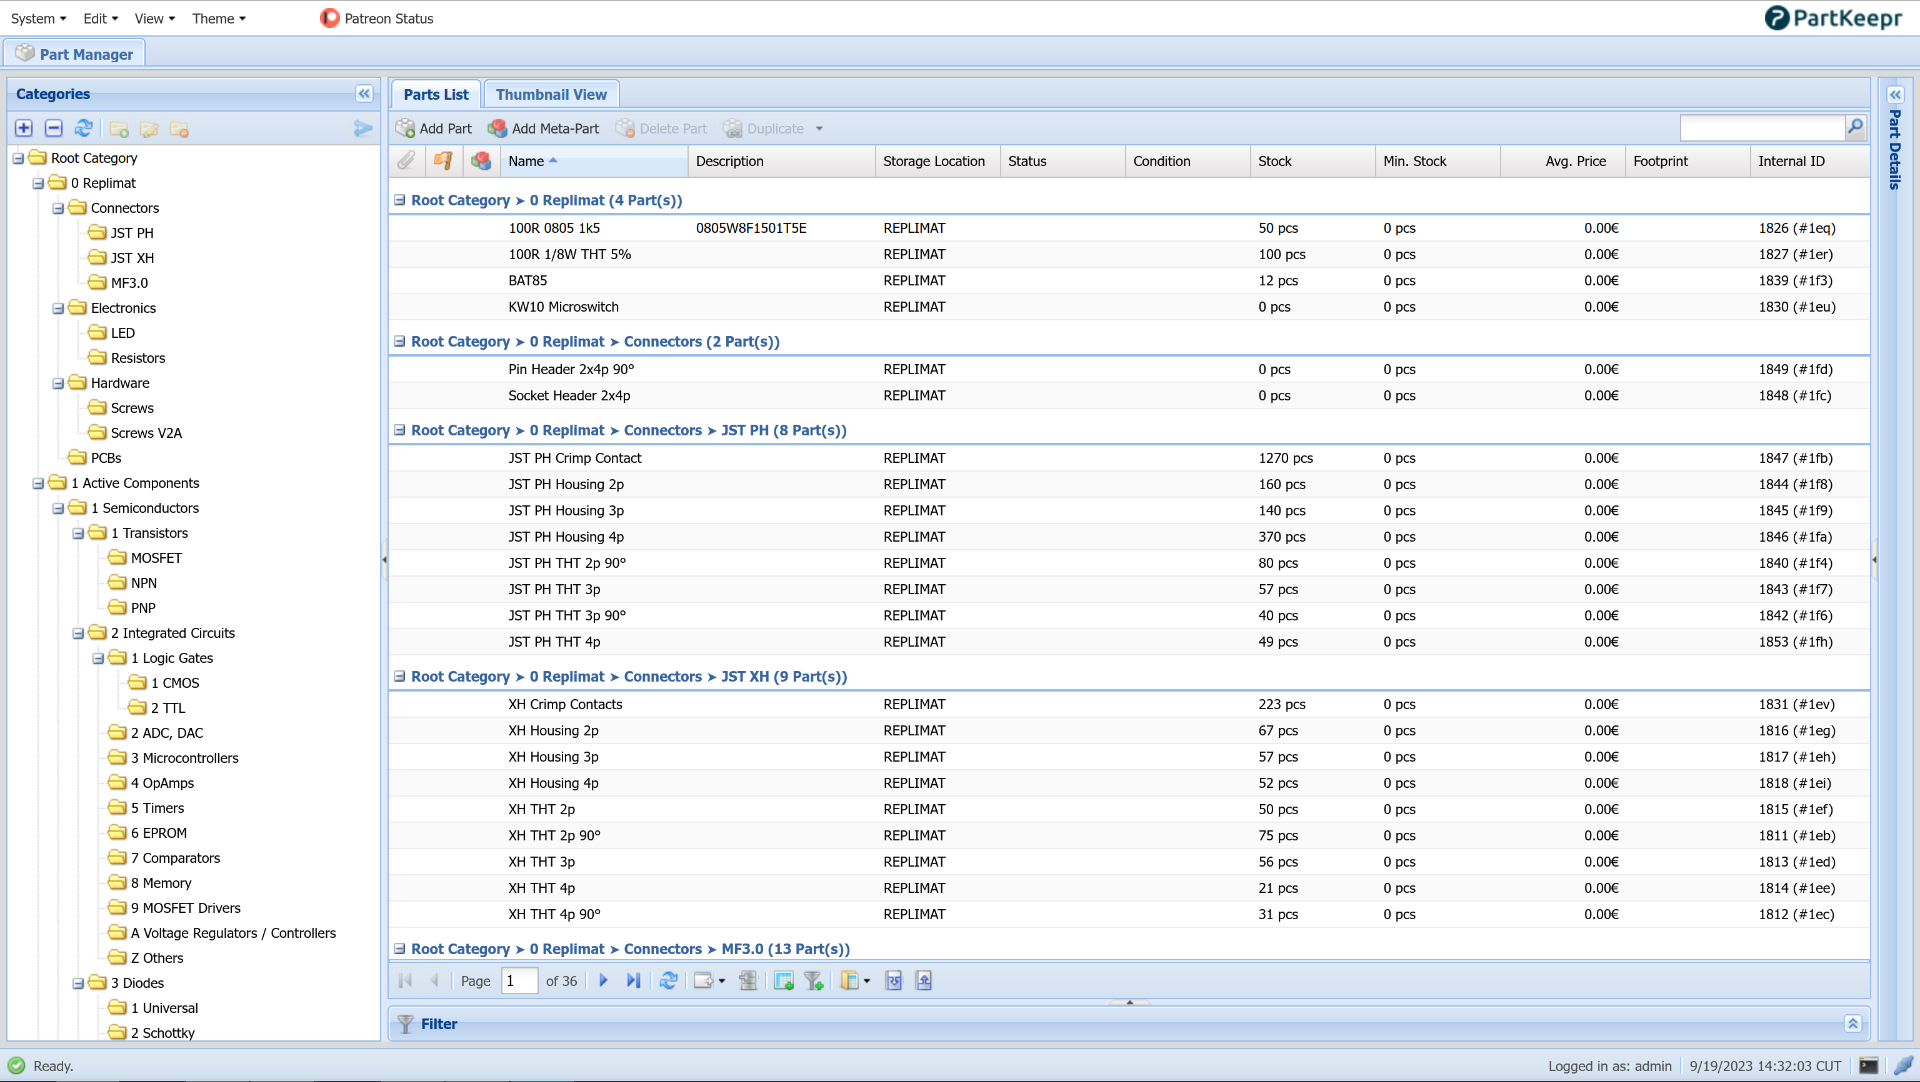
\includegraphics[width=15cm]{partkeepr_demo_homepage.png}

\subparagraph[indent=false]{Overview}

\noindent \\PartKeepr is an open-source inventory management system with a focus on electronic components.
It is designed around four main principles:

\begin{outline}
    \1 Fast Part Searching
    \1 Ability to add complete part database
    \1 Keeping track of stock
    \1 Ease of use
\end{outline}

\subparagraph{Parts applicable to my solution\\}

\noindent Like PartKeepr, I hope to implement a web-based interface.
However, I am using a different approach as my solution will not be tailored specifically to electronic components.

\pagebreak

% 3. Sortly
\paragraph{Sortly}
\url{https://www.sortly.com/solutions/inventory-management-software/}\\

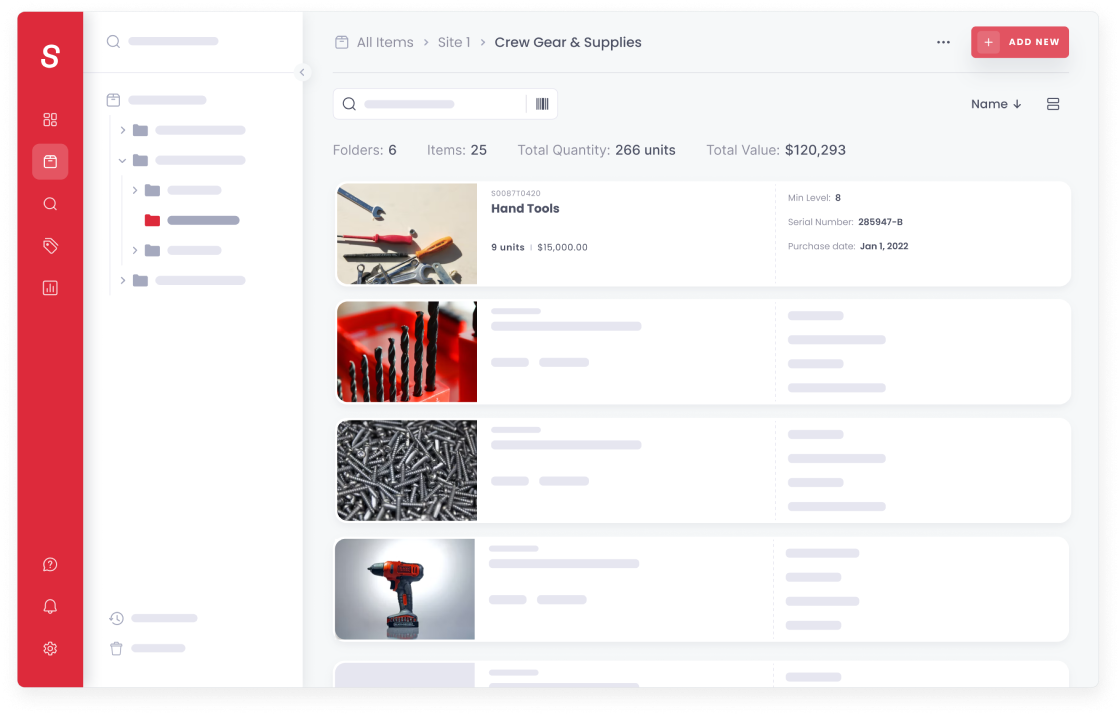
\includegraphics[width=15cm]{sortly_homepage_mockup_1.png}

\subparagraph{Overview}

\noindent \\Sortly is a proprietary cloud-based inventory management system with a focus on small businesses and inviduals.\\\\
It has two plans available, an always free plan with limited functionality and a paid plan will a more complete feature-set.

\subparagraph{Parts applicable to my solution\\}

I hope to implement the following features from Sortly:

\begin{outline}
    \1 Web based interface
    \2 Allows for easy access.

    \1 Barcode support
    \2 Allows end users to print off QR codes to stick to items
    \2 Which can be scanned in-app to easily perform actions on the item.

    \1 Real-time reporting insights
    %\subitem 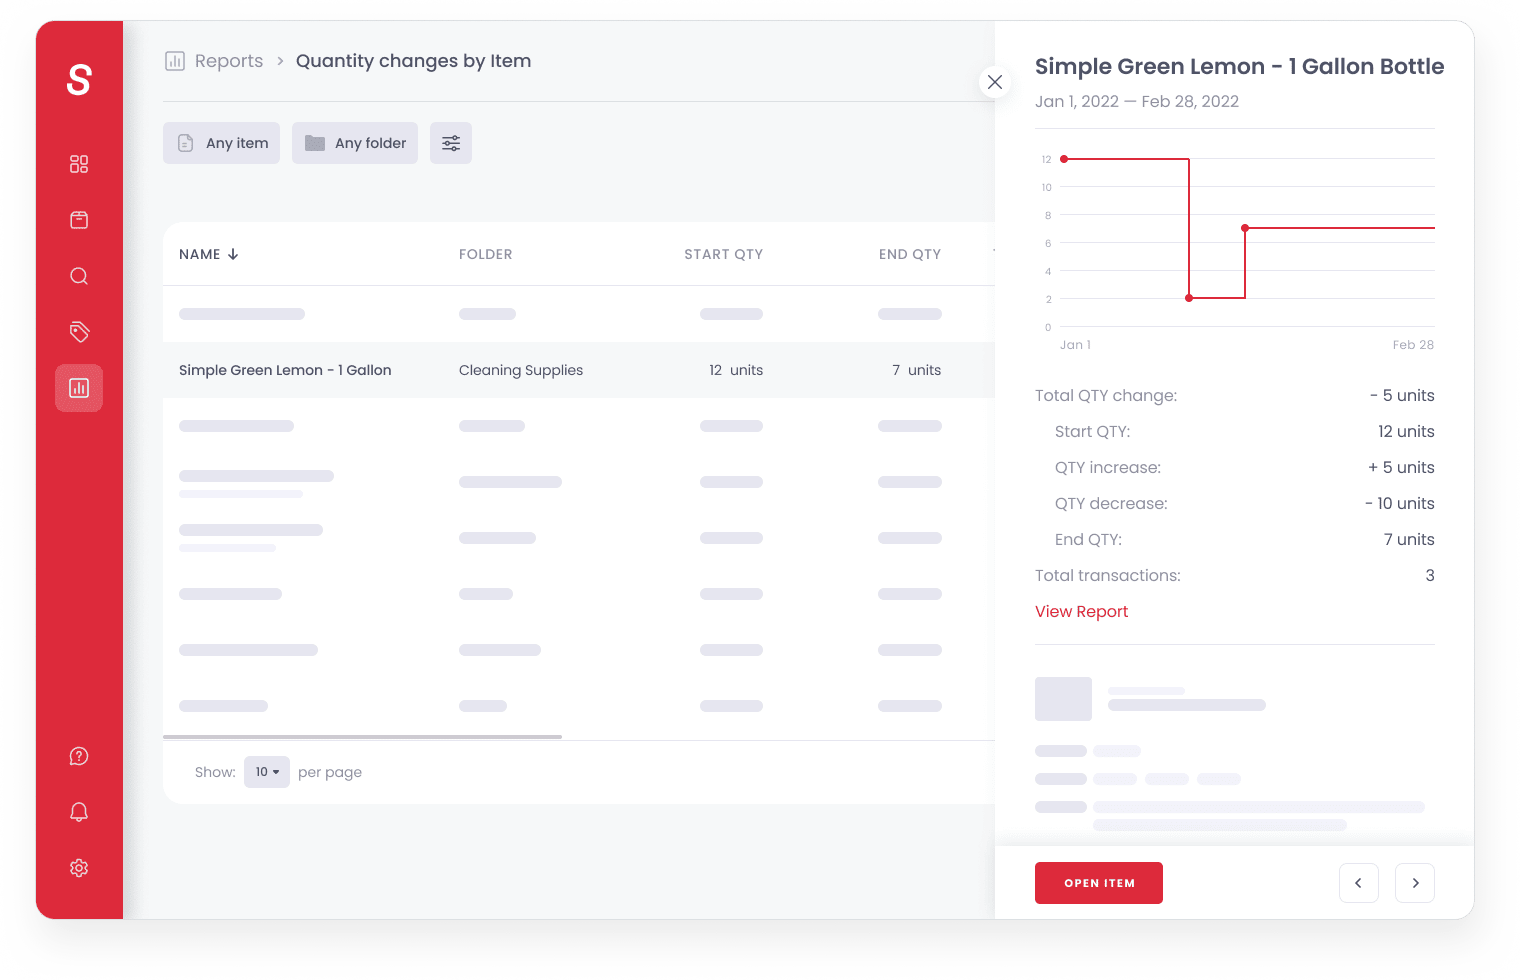
\includegraphics[width=10cm]{sortly_homepage_mockup_2.png}
    \2 Allows for added insight into usage patterns for particular units.
\end{outline}

\pagebreak

\paragraph{Koha\\}
\url{https://koha-community.org/}

\subparagraph{Overview}

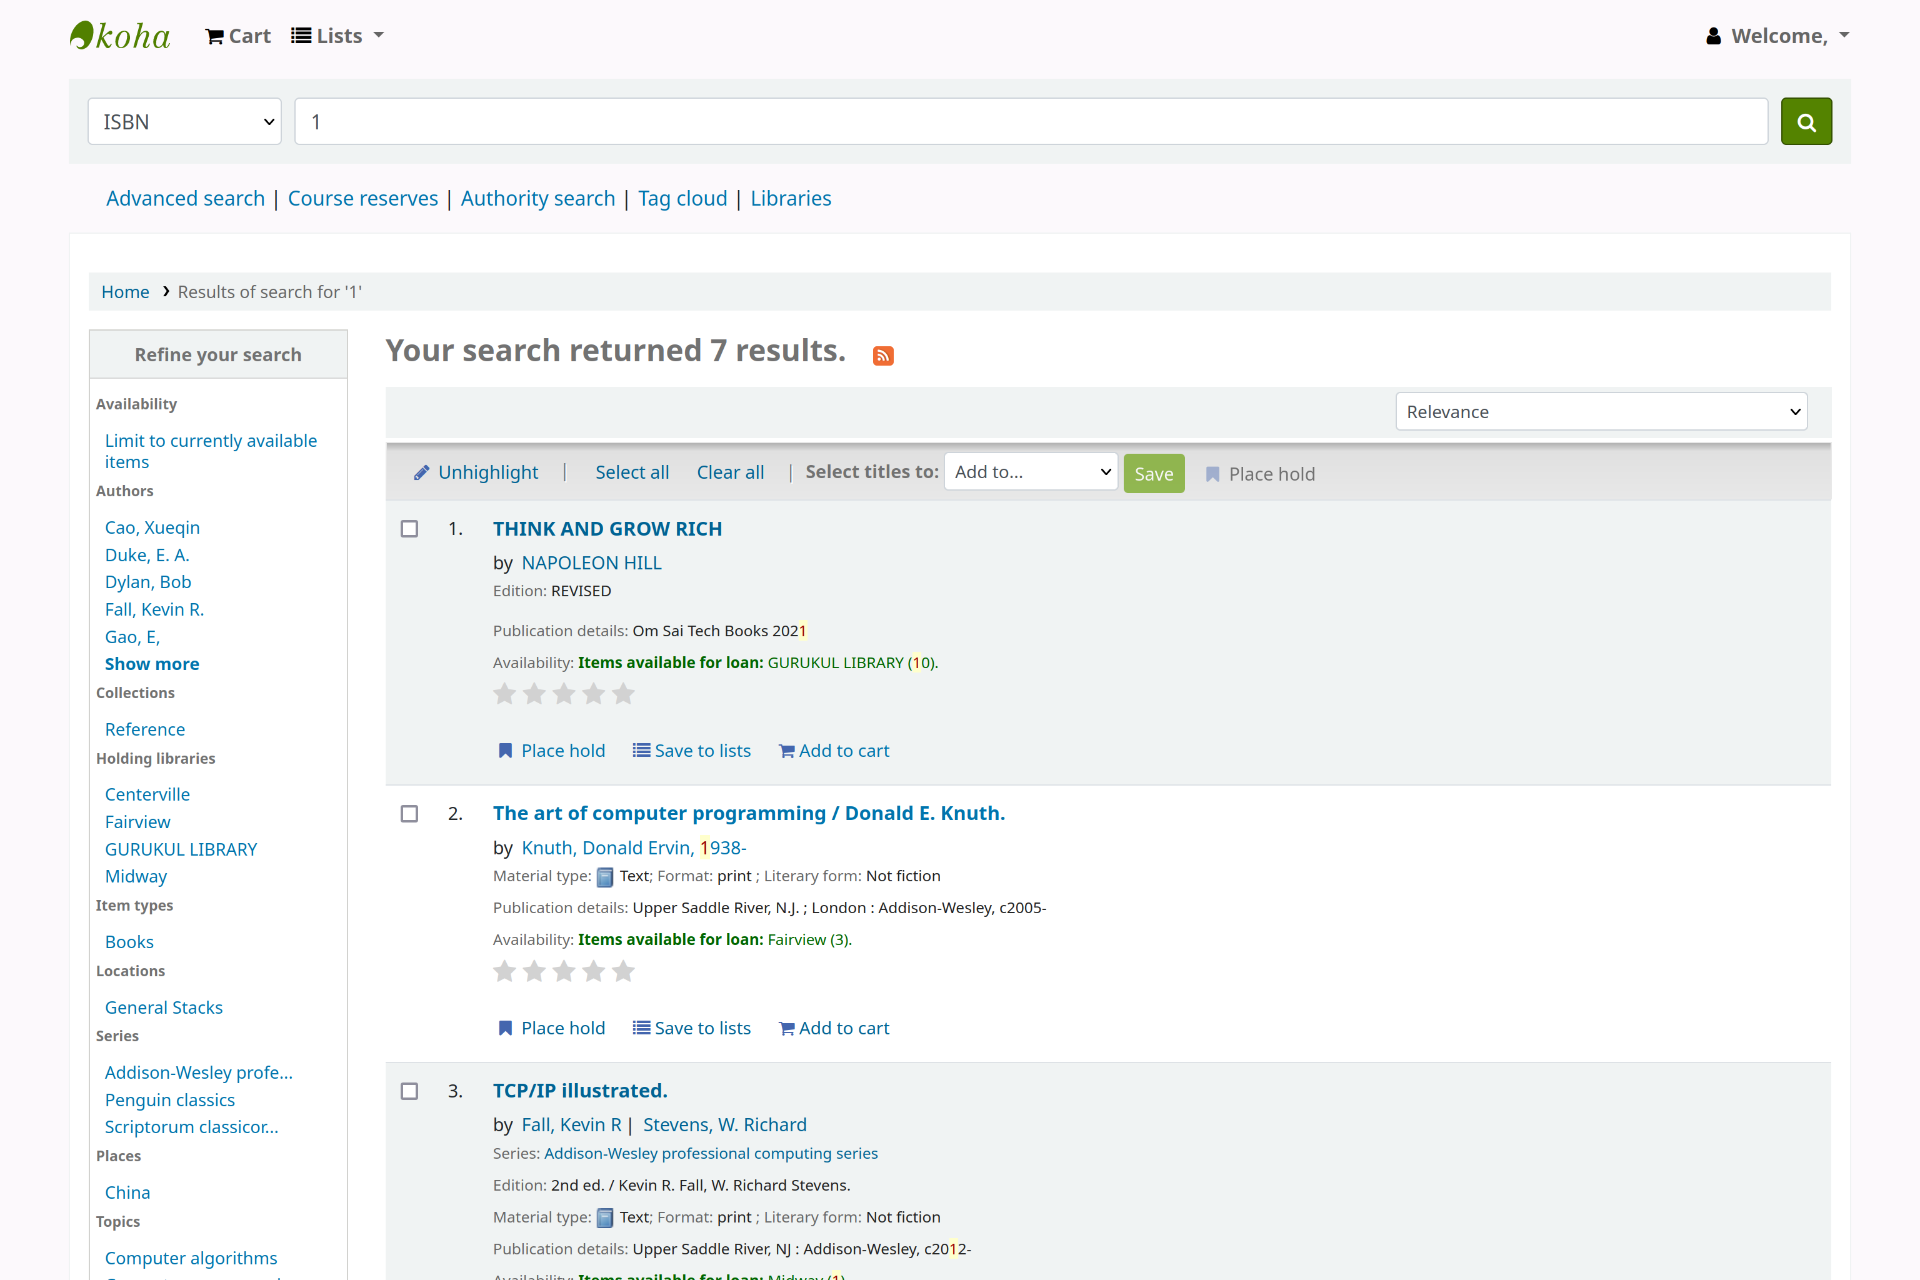
\includegraphics[width=15cm]{koha_demo_searching.png}

\subparagraph{Parts applicable to my solution\\}
\subparagraph{Parts \underline{not} applicable to my solution\\}

\end{document}